% 040_asymmetry_cost_curve.tex
% Conceptual illustration of asymmetric cost penalties

\begin{figure}[h!]
\centering
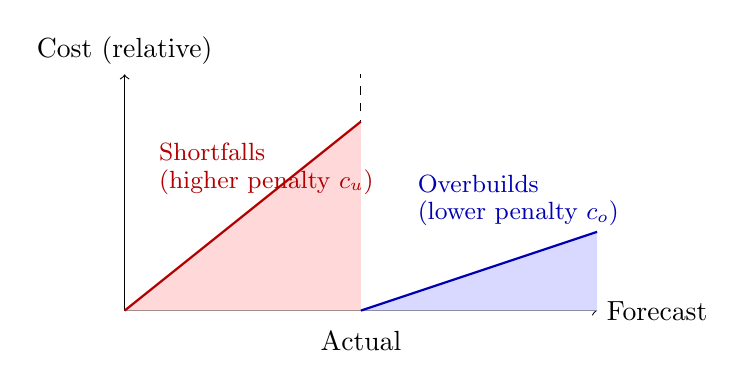
\begin{tikzpicture}[scale=1]

  % Axes
  \draw[->] (0,0) -- (6,0) node[right] {Forecast};
  \draw[->] (0,0) -- (0,3) node[above] {Cost (relative)};

  % Vertical line at Actual
  \draw[dashed] (3,0) -- (3,3);
  \node[below=4pt] at (3,0) {Actual};

  % Shortfall region
  \fill[red!15] (0,0) -- (3,0) -- (3,2.4) -- cycle;
  \draw[red!70!black, thick] (0,0) -- (3,2.4);
  \node[red!70!black, align=left] at (1.8,1.8)
      {\small Shortfalls\\[-2pt]\small (higher penalty $c_u$)};

  % Overbuild region
  \fill[blue!15] (3,0) -- (6,0) -- (6,1.0) -- cycle;
  \draw[blue!70!black, thick] (3,0) -- (6,1.0);
  \node[blue!70!black, align=left] at (5.0,1.4)
      {\small Overbuilds\\[-2pt]\small (lower penalty $c_o$)};

\end{tikzpicture}
\caption{Conceptual illustration of asymmetric penalties: shortfalls incur a higher
penalty ($c_u$) than overbuilds ($c_o$).}
\label{fig:asymmetry}
\end{figure}